\hypertarget{models-dynamical-systems-and-filters}{%
\section{Models, Dynamical Systems and
Filters}\label{models-dynamical-systems-and-filters}}

In this section we learn how to model the dynamics of the system. For
our purposes, it is sufficient to use a simplified model of the
dynamics. We will assume that the system dynamics are linear and the
variations in the dynamics (the noise) is normal or Gaussian. We will
immediately see that this assumptions leaves out the most basic of our
robot models, the differential drive. Our resolution will be to develop
the theory with the linear Gaussian systems and then develop ways to
adapt it to real systems.

\hypertarget{creating-filters-from-data-and-models}{%
\subsection{Creating Filters from data and
models}\label{creating-filters-from-data-and-models}}

Say that you have a lidar at the side a road or railway which you intend
to track velocity of the passing vehicle.\footnote{Ignoring for the
  moment that this is a ridiculously expensive way to track velocity.}
The lidar will estimate the distance at the various sweep angles. This
can be converted from the polar coordinates of the lidar to the
rectangular coordinates natural for tracking the vehicle. Because of
measurement error in \((r, \theta)\), you have a distribution of
possible values in \((x,y)\) of the actual vehicle state (location). If
you did not have any additional information, you would have to report
the measurement and the standard deviations (assuming you believe the
error is normally distributed), and be done.

However, in this case you do have some additional information. Focusing
on the train, you know the vehicle is restricted to the rail. This
information can be used to reduce or filter out some of the error. The
idea then would be to project the estimate of location onto the track
since you know (well actually assume) the restriction of the vehicle.
The rail here is our proxy for kinematic constraints. The kinematic
constraints describes the restrictions on motion just like the rail
restricts the train motion. It makes sense then to use the kinematics to
help filter out the noise in our measurements.

\hypertarget{measurement-to-model-to-estimatepredict}{%
\subsubsection{\texorpdfstring{Measurement \(\to\) Model \(\to\)
Estimate/Predict}{Measurement \textbackslash to Model \textbackslash to Estimate/Predict}}\label{measurement-to-model-to-estimatepredict}}

The work we did earlier in fitting curves is one form of this idea. We
have a model in mind and we then ``project'' the data onto the model.

\begin{figure}
\centering
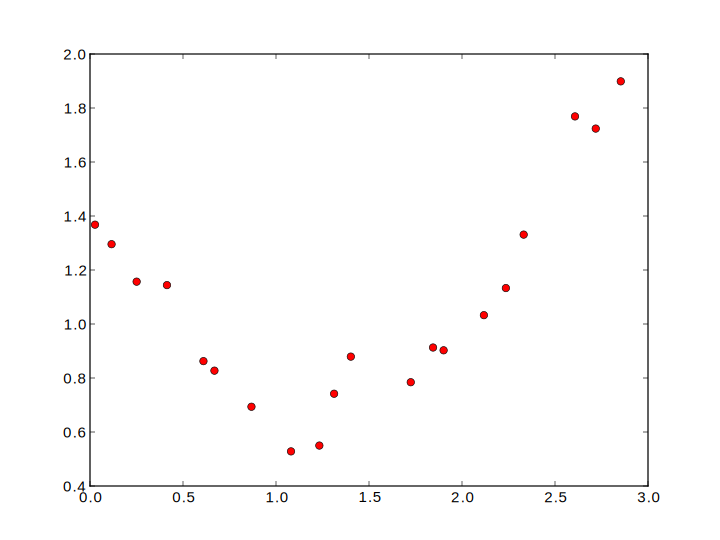
\includegraphics[width=0.6\textwidth,height=\textheight]{AdvFilteringFigures/quadpts.*}
\caption{}
\end{figure}

~\(\Rightarrow\)

\begin{figure}
\centering
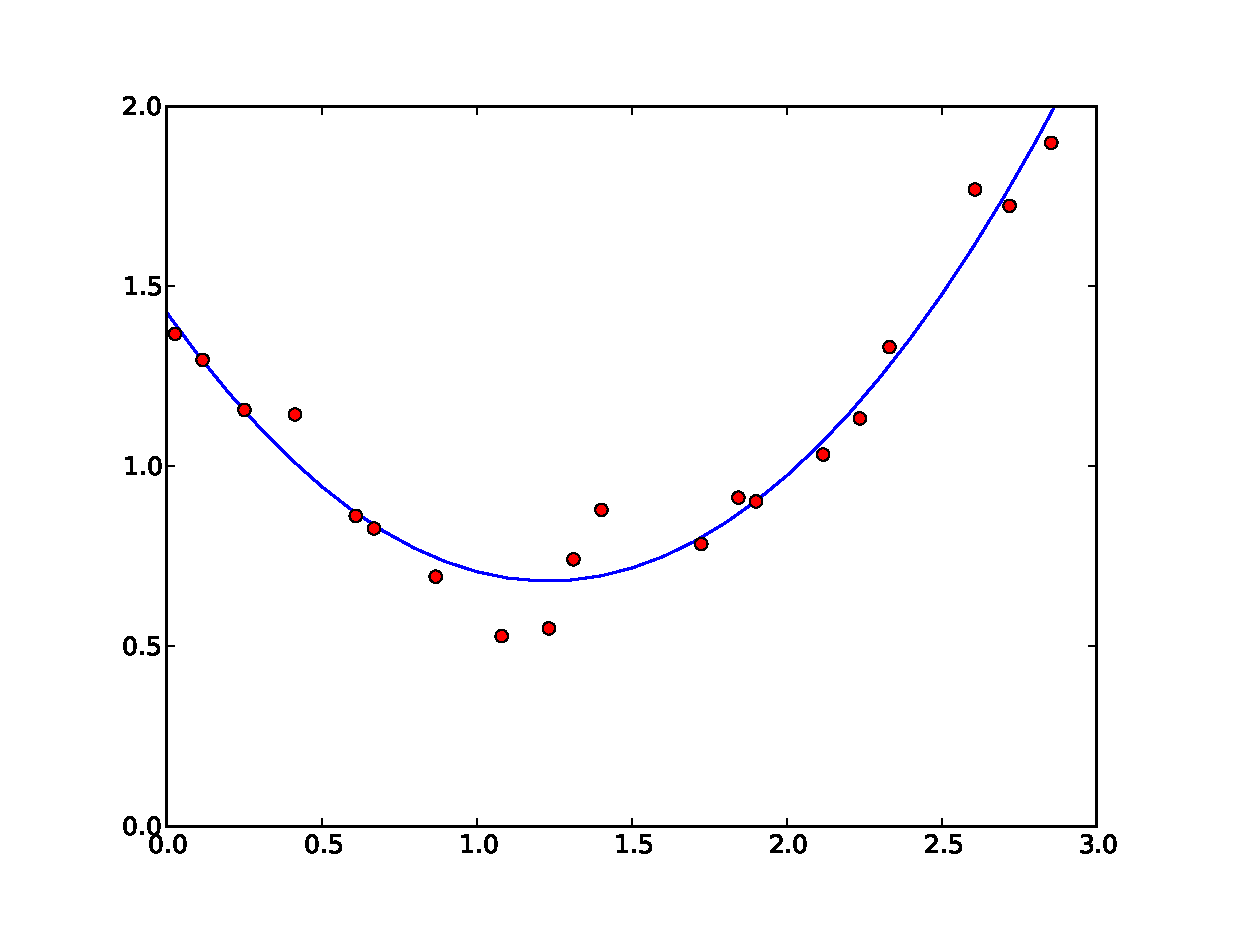
\includegraphics[width=0.6\textwidth,height=\textheight]{AdvFilteringFigures/quadgraph.*}
\caption{}
\end{figure}

Using quadratic model, \(y = c_2x^2 + c_1x + c_0\), and least squares we
find \(y = 0.49x^2 - 1.21x + 1.42\). So we can use this to extrapolate
at \(x=5\) we have \(y = 6.5\).

\begin{figure}
\centering
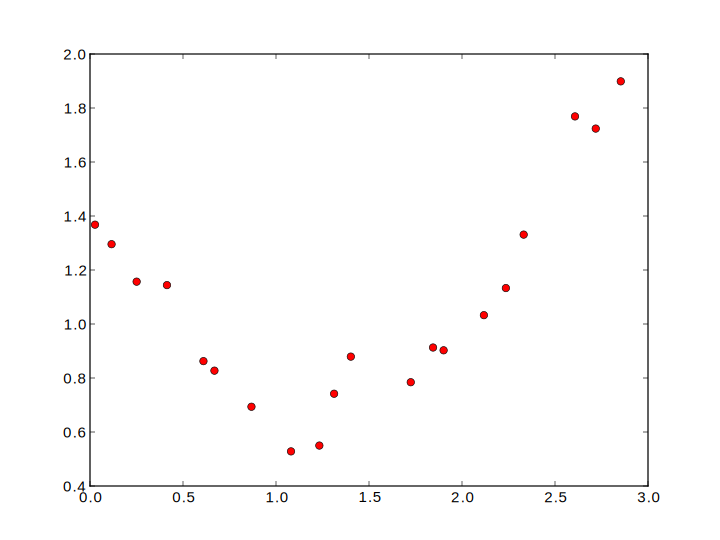
\includegraphics[width=0.6\textwidth,height=\textheight]{AdvFilteringFigures/quadpts.*}
\caption{}
\end{figure}

~\(\Rightarrow\)

\begin{figure}
\centering
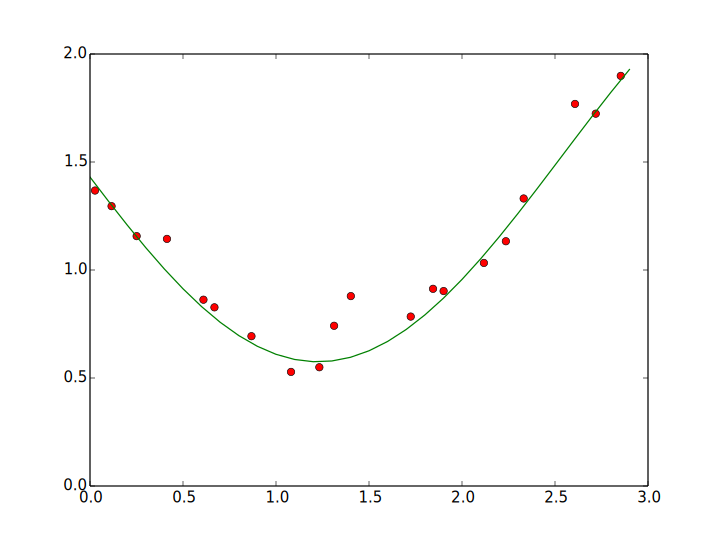
\includegraphics[width=0.6\textwidth,height=\textheight]{AdvFilteringFigures/lscompare.*}
\caption{}
\end{figure}

Note that this is very different from using a sinusoidal model and
gaining the fit \(y= -0.95\sin(1.2x+0.1)+1.525\), where for \(x=5\) we
have \(y=1.698\)

\hypertarget{a-physics-example}{%
\subsubsection{A Physics Example}\label{a-physics-example}}

In this example, we go one step further. Using observational data of
motion and knowing the motion is restricted in some manner, can we then
use the data + model to predict a missing piece of information. Formally
this is known as interpolation or extrapolation depending on the
dataset. We use the data plus the model to answer the question. Physical
systems have equations describing the behavior of the objects in the
system. For example one may know about the forces acting on an object of
mass \(m\), \(F_x\) and \(F_y\) which will give the equations of motion

\[\ddot{x} = \frac{F_x}{m} \quad \quad \ddot{y} = \frac{F_y}{m} .\]

For this example, assume that these forces are constant and so we may
easily integrate them

\[x(t) =  \frac{F_x}{2m} t^2 + v_{x,0} t + x_0 \quad \mbox{and} \quad y(t) =  \frac{F_y}{2m} t^2 + v_{y,0} t + y_0 .\]

These equations restrict the possible values of \(x\) and \(y\) while
still being general enough to allow for a variety of starting
conditions. Assume for the moment that we do not have knowledge of the
initial data for a particular application (but understand the forces
involved) and would like to use some observed data to determine those
values. The observations of the moving object are probably very noisy.
Thus you would obtain \((t_i, x_i,y_i)\) data (\(i=1 \dots k\)). Each
data item should satisfy the equations

\[x_i =  \frac{F_x}{2m} t_i^2 + v_{x,0} t_i + x_0 \quad \mbox{and} \quad y_i =  \frac{F_y}{2m} t_i^2 + v_{y,0} t_i + y_i, \quad i=1 \dots k .\]

There are two unknowns for each equation. Two data points would allow an
exact answer (two equations and two unknowns). But what if you had a
dozen observations? With noisy data, getting many observations should
provide a better estimate of the initial values than just picking two
observed values. So, how do we do this?

We assume that we have obtained some data on the motion of an object and
wish to compute its equations of motion. Plugging the data in gives the
equations:

\[x_i =  \frac{F_x}{2m} t_i^2 + v_{x,0} t_i + x_0 \quad \mbox{and} \quad y_i =  \frac{F_y}{2m} t_i^2 + v_{y,0} t_i + y_i, \quad i=1 \dots k .\]

Rewrite the expression as

\[\xi_i = x_i -  \frac{F_x}{2m} t_i^2 = v_{x,0} t_i + x_0 \quad \mbox{and} \quad \eta_i = y_i -  \frac{F_y}{2m} t_i^2 = v_{y,0} t_i + y_i, \quad i=1 \dots k .\]

Then

\[\begin{aligned}
\begin{pmatrix} \xi_1 \\ \xi_2 \\ \dots \\ \xi_k \end{pmatrix} = \begin{pmatrix} t_1 & 1 \\ t_2 & 1 \\ \vdots & \vdots \\ t_k & 1 \end{pmatrix} \begin{pmatrix}  v_{x,0} \\ x_0 \end{pmatrix}
\quad \mbox{and} \quad
\begin{pmatrix} \eta_1 \\ \eta_2 \\ \dots \\ \eta_k \end{pmatrix} = \begin{pmatrix} t_1 & 1 \\ t_2 & 1 \\ \vdots & \vdots \\ t_k & 1 \end{pmatrix} \begin{pmatrix}  v_{y,0} \\ y_0 \end{pmatrix}
\end{aligned}\]

The pseudo-inverse is \(M = (X^T X)^{-1} X^T\)

\[\begin{aligned}
=  \left[\begin{pmatrix} t_1 & t_2 & \dots & t_k  \\ 1 & 1 & \dots & 1\end{pmatrix} \begin{pmatrix} t_1 & 1 \\ t_2 & 1 \\ \vdots & \vdots \\ t_k & 1 \end{pmatrix} \right]^{-1}
\begin{pmatrix} t_1 & t_2 & \dots & t_k  \\ 1 & 1 & \dots & 1\end{pmatrix}
\end{aligned}\]

which gives the least squares estimate

\[\begin{aligned}
\begin{pmatrix}  v_{x,0} \\ x_0 \end{pmatrix} =  M  \begin{pmatrix} \xi_1 \\ \xi_2 \\ \dots \\ \xi_k \end{pmatrix}
\quad \mbox{and}
\quad
\begin{pmatrix}  v_{y,0} \\ y_0 \end{pmatrix} =
M \begin{pmatrix} \eta_1 \\ \eta_2 \\ \dots \\ \eta_k \end{pmatrix}
\end{aligned}\]

\hypertarget{physics-example-with-numbers}{%
\subsubsection{Physics example with
numbers}\label{physics-example-with-numbers}}

Assume that we had the following data:
\((t,x,y) =  (1, 10, 22), (2, 19, 60), (3, 32,
51)\) and that \(F_x=0\) and \(F_y = -2\), \(m=0.25\). So first we gain:
\(t = [1, 2, 3]\), \(\xi = [10, 19, 32]\), \(\eta = [26, 76, 87]\). We
first compute

\[\begin{aligned}
\left[\begin{pmatrix} 1 & 2 &  3  \\ 1 & 1 & 1\end{pmatrix} \begin{pmatrix} 1 & 1 \\ 2 & 1  \\ 3 & 1 \end{pmatrix} \right]^{-1}
= \left[\begin{pmatrix} 14 & 6 \\ 6 & 3 \end{pmatrix}\right]^{-1} =  \frac{1}{6} \begin{pmatrix} 3 & -6 \\ -6 & 14 \end{pmatrix}
\end{aligned}\]

\[\begin{aligned}
= \begin{pmatrix} 1/2 & -1 \\ -1 & 7/3 \end{pmatrix}
\end{aligned}\]

\[\begin{aligned}
\begin{pmatrix}  v_{x,0} \\ x_0 \end{pmatrix} = \begin{pmatrix} 1/2 & -1 \\ -1 & 7/3 \end{pmatrix}
\begin{pmatrix} 1 & 2 &  3  \\ 1 & 1 & 1\end{pmatrix}  \begin{pmatrix} 10 \\ 19 \\ 32 \end{pmatrix}  = \begin{pmatrix} 11 \\ -1.666667\end{pmatrix}
\end{aligned}\]

and

\[\begin{aligned}
\begin{pmatrix}  v_{y,0} \\ y_0 \end{pmatrix} = \begin{pmatrix} 1/2 & -1 \\ -1 & 7/3 \end{pmatrix}
\begin{pmatrix} 1 & 2 &  3  \\ 1 & 1 & 1\end{pmatrix} \begin{pmatrix} 26 \\ 76 \\ 87\end{pmatrix} = \begin{pmatrix} 30.5 \\ 2.0\end{pmatrix}
\end{aligned}\]

So we have that the start location is \((-1.666667, 2.0)\) with initial
velocity of \((11 , 30.5)\).

\hypertarget{linear-dynamical-system}{%
\subsection{\texorpdfstring{\texttt{Linear\ Dynamical\ System}}{Linear Dynamical System}}\label{linear-dynamical-system}}

An operator, \(L\), is said to be \texttt{linear} if for scalars \(a,b\)
and vectors \(x,y\) we have

\[L(ax+by) = aLx + bLy\]

A \texttt{dynamical\ system}

\[x_k = Lx_{k-1} \quad \text{(discrete)}\]

or

\[\dot{x} = Lx \quad \text{(continuous)}\]

is said to be linear if \(L\) is a linear operator. Linearity means we
may construct solutions using simple addition.

\hypertarget{example-of-linear-operators}{%
\subsubsection{Example of linear
operators}\label{example-of-linear-operators}}

Some examples of linear operators are matrices,
\(A(\alpha x + \beta y) = \alpha Ax + \beta Ay\), and derivatives,
\((d/dx) [\alpha u+\beta v] = \alpha du/dx + \beta dv/dx\).

\hypertarget{example-nonlinear-kinematic-models}{%
\subsubsection{Example: Nonlinear Kinematic
Models}\label{example-nonlinear-kinematic-models}}

The dynamics of a differential drive robot is \textbf{NOT} linear:

\[\begin{aligned}
\begin{array}{l}
 \dot{x} = \frac{r}{2} (\dot{\phi_1}+\dot{\phi_2})\cos(\theta) \\[5mm]
\dot{y} = \frac{r}{2} (\dot{\phi_1}+\dot{\phi_2})\sin(\theta) \\[5mm]
\dot{\theta} = \frac{r}{2L} (\dot{\phi_1}-\dot{\phi_2}).
\end{array}
\end{aligned}\]

This follows from noting that \(\cos(\theta)\) and \(\sin(\theta)\) are
nonlinear functions of the state variable \(\theta\).

\hypertarget{dynamics-with-noise}{%
\subsection{Dynamics with Noise}\label{dynamics-with-noise}}

Let \(x_k\) be the current state and \(z_k\) be the observation. We
study the linear system with noise:

\[\begin{aligned}
\begin{array}{l}
x_k = Fx_{k-1} + Gu_k + v_k\\
z_k = Hx_k + w_k
\end{array}
\end{aligned}\]

where \(v_k\), \(w_k\) are assumed to be zero mean Gaussian noise with
covariance matrices \(V_k\) and \(W_k\) respectively.

We are interested in tracking not just the estimate of the state, but
the state's distribution as well since the addition of noise produces
random variations in values. The simplest distribution to track is a
Normal or Gaussian distribution. Using the Bayes Filter terminology, we
have three elements:

\begin{enumerate}
\item
  The state transition probability \(p(x_k|u_k,x_{k-1})\) must arise
  from

  \[x_k = Fx_{k-1}+Gu_k + v_k\]

  where \(x_k\), \(x_{k-1}\) are state vectors, \(u_k\) controls,
  \(v_k\) is the noise, \(F\) and \(G\) are matrices. \(v_k\) is a mean
  zero normally distributed random variable with covariance matrix
  \(V_k\). This is linear system dynamics. Thus the mean of the
  posterior state is

  \[E(x_k) =
  Fx_{k-1}+Gu_k,\]
\end{enumerate}

\(p(x_k|u_k, x_{k-1})\)

\begin{quote}
\[= \frac{1}{\sqrt{\det
    (2\pi V_k)}}e^{-\frac{1}{2}(x_k-Fx_{k-1}-Gu_k)^T V^{-1}(x_k-Fx_{k-1}-Gu_k)}.\]
\end{quote}

\begin{enumerate}
\item
  The measurement probability \(p(z_k|x_k)\) must also be linear

  \[z_k = Hx_k + w_k\]

  where \(H\) is a \(m \times n\) matrix and \(w_k\) is Gaussian mean
  zero random variable (noise) with covariance matrix \(W_k\). The mean
  of the observation

  \[E(z_k) = Hx_k,\]

  \[p(z_k|x_k) = \frac{1}{\sqrt{\det
      (2\pi W_k)}}e^{-\frac{1}{2}(z_k-Hx_k)^T W^{-1}(z_k-Hx_k)}\]
\item
  Initial belief, \(\mbox{bel}(x_0)\) must be normally distributed, say
  with mean \(\hat{x}_0\) and covariance \(P_0\)

  \[\mbox{bel}(x_0) = \frac{1}{\sqrt{\det
      (2\pi P_0)}}e^{-\frac{1}{2}(x_0-\hat{x}_0)^T P_0^{-1}(x_0-\hat{x}_0)}\]

  If assumptions 1,2,3 hold then \(\mbox{bel}(x_k)\) is also a Gaussian
  distribution.
\end{enumerate}

\hypertarget{terminology}{%
\subsubsection{Terminology}\label{terminology}}

We will introduce some fairly common notation used in state estimation.
As stated before, we cannot observe the actual value of the quantity
\(x\), and so we will indicate with a ``hat'' the estimate of the value,
\(\hat{x}\).

\begin{itemize}
\tightlist
\item
  Let \(\hat{x}_{k-1|k-1}\) be the current state estimate at time step
  \(k-1\).
\item
  Let \(\hat{x}_{k|k-1}\) be the prediction of the next state using a
  model of the dynamics.
\item
  Let \(P_{k|k-1}\) be the covariance of \(\hat{x}_{k|k-1}\)
  (\(E[(x_k-\hat{x}_{k|k-1})(x_k-\hat{x}_{k|k-1})^T]\))
\item
  Let \(z_{k}\) be the observation or measurement of \(x_{k}\).
\item
  Let \(\hat{x}_{k|k}\) be the update based on the observation.
  \(\hat{x}_{k|k}\) is our best estimate of \(x_{k}\)
\item
  Let \(P_{k|k}\) be the covariance of \(\hat{x}_{k|k}\)
  (\(E[(x_k-\hat{x}_{k|k})(x_k-\hat{x}_{k|k})^T]\))
\item
  Let \(V_k\) be the process noise covariance matrix.
\item
  Let \(W_k\) be the observation noise covariance matrix.
\end{itemize}

At the risk of being redundant, we need to address a common
misunderstanding. The state vector \(x\) is not something that normally
can be observed. We would not need to do any type of filtering if we
could observe it. The observation of \(x\) is \(z\). It differs from
\(x\) in two primary manners. First there is noise in the observation.
Meaning that \(x\) and \(z\) differ by the added noise. Second, we don't
observe all of the components of \(x\). Some are missing. This means
that the lengths of the vectors for \(x\) and \(z\) are often different.

For the algorithms in the next couple of sections, we will be estimating
\(x\) by using \(z\). So \(z\) is an input variable. To develop code, we
need to test on actual data sets, so we will need to create some fake
\(z\) to run our tests. The creation of the \(z\) data is not part of
any of the filters. This is no different than when you create unit
tests. They are essential to the development process, but not part of
the primary codebase.

\hypertarget{scalar-kalman-filter}{%
\subsection{\texorpdfstring{\texttt{Scalar\ Kalman\ Filter}}{Scalar Kalman Filter}}\label{scalar-kalman-filter}}

For the moment assume that \(x, F, G, u\) are scalars. Also assume we
have a starting value for the state \(x_0\) and some estimate of the
error in that starting value, \(\sigma_0^2\). The error in the process
is measured and has variance \(\sigma_v^2\), meaning \(v_k\) is drawn
from a zero mean Gaussian distribution with variance \(\sigma_v^2\)
which gives us the process:

\[x_k = Fx_{k-1} + Gu_k  + v_k .\]

The estimate of state based on the process is simply

\[\tilde{x}_k = F\hat{x}_{k-1} + Gu_k .\]

Prior to the process, the variance estimate for \(x_{k-1}\) is
\(\sigma_{k-1}^2\). What happens? It is transformed via

\[\tilde{\sigma}_{k}^2 = (F \sigma_{k-1})^2 + \sigma_v^2 = F^2\sigma_{k-1}^2 + \sigma_v^2 .\]

The next thing required is to merge the process prediction with the
observation data, \(z_k\) (scalar), this observation has quality
\(\sigma_w^2\). These are fused using \texttt{scalarrecursiveweighted}
into

\[S_k = \frac{1}{\tilde{\sigma}_k^2} + \frac{1}{{\sigma}_w^2}\]

\[K_{k} = \displaystyle \left[ S_{k}\sigma_{w}^2\right]^{-1} =  \left[ {\sigma}_{w}^2 \left(\frac{1}{\tilde{\sigma}_k^2} + \frac{1}{\sigma_w^2}\right) \right]^{-1}
=  \left[ {\sigma}_{w}^2 \left(\frac{\tilde{\sigma}_k^2 + \sigma_w^2}{\tilde{\sigma}_k^2  \sigma_w^2}\right) \right]^{-1}\]

\[=  \frac{\tilde{\sigma}_k^2}{\tilde{\sigma}_k^2 + \sigma_w^2}\]

\[\hat{x}_{k} =  \tilde{x}_{k-1} +  K_{k}\left(  z_{k}- \tilde{x}_{k-1} \right)\]

\[\displaystyle \sigma_k^{2} = (1 - K_k)\tilde{\sigma}_k^{2}\]

We can summarize the process

\[\begin{aligned}
\begin{array}{l}
x_k = Fx_{k-1} + Gu_k + v_k\\
z_k = x_k + w_k
\end{array}
\end{aligned}\]

in the standard notation of the Kalman Filter. Let the process noise
\(v_k\) have variance \(V = \sigma_v^2\) and the observation noise
\(w_k\) have variance \(W = \sigma_w^2\). We track the estimate (or
mean) \(\hat{x}_{k|k}\) and the variance \(p_{k|k}\). We will also make
the following substitutions: \(P_{k-1|k-1} = \sigma_{k-1}^2\),
\(P_{k|k-1} = \tilde{\sigma}_k^2\) and \(P_{k|k} = \sigma_{k}^2\).

\hypertarget{the-scalar-kalman-filter-algorithm}{%
\subsubsection{The Scalar Kalman Filter
Algorithm}\label{the-scalar-kalman-filter-algorithm}}

In the case where the state vector to be estimated is a scalar, the
derivation is much easier and sets the stage for the multivariate
version shown in the next section.

\begin{itemize}
\tightlist
\item
  Predicted state: \(\hat{x}_{k|k-1} = F\hat{x}_{k-1|k-1} + G u_{k}\)
\item
  Predicted estimate error: \(P_{k|k-1} = F^2 P_{k-1|k-1}  + V\)
\item
  Optimal Kalman gain: \(K_k = P_{k|k-1}/( P_{k|k-1}  + W)\)
\item
  Updated state estimate
  \(\hat{x}_{k|k} =\hat{x}_{k|k-1} + K_k (z_k - \hat{x}_{k|k-1})\)
\item
  Updated estimate variance: \(P_{k|k} = (1 - K_k) P_{k|k-1}\)
\end{itemize}

\hypertarget{example}{%
\subsubsection{Example}\label{example}}

Assume that you are given a simple scalar process on \(0 \leq k < N\):

\[x_k = x_{k-1} + u_k\]

where the control input is

\[u_k = 0.5*(1 - 1.75k/N).\]

Also assume that you have process noise with standard deviation of
\(0.2\) and observation noise with standard deviation of \(0.75\).

When we don't have actual experimental data, we need to simulate the
data. To illustrate the filter, we will create a noisy dataset; we
pretend to run the dynamical system and get the observations. Later on
in the multivariate content, much greater detail is given to the
creation of noisy data. For now, focus on the filter aspect and not on
the creation of \(z\).

\begin{Shaded}
\begin{Highlighting}[]
\KeywordTok{using}\NormalTok{ Plots}\OperatorTok{,} \BuiltInTok{Random}\OperatorTok{,}\NormalTok{ Distributions}

\NormalTok{N }\OperatorTok{=} \FloatTok{100}
\NormalTok{mu1}\OperatorTok{,}\NormalTok{ sigma1 }\OperatorTok{=} \FloatTok{0.0}\OperatorTok{,} \FloatTok{0.2}
\NormalTok{mu2}\OperatorTok{,}\NormalTok{ sigma2 }\OperatorTok{=} \FloatTok{0.0}\OperatorTok{,} \FloatTok{0.75}
\NormalTok{r1 }\OperatorTok{=}\NormalTok{ Normal(mu1}\OperatorTok{,}\NormalTok{ sigma1)}
\NormalTok{r2 }\OperatorTok{=}\NormalTok{ Normal(mu2}\OperatorTok{,}\NormalTok{ sigma2)}

\NormalTok{process\_noise }\OperatorTok{=}\NormalTok{ rand(r1}\OperatorTok{,}\NormalTok{N)}
\NormalTok{observation\_noise }\OperatorTok{=}\NormalTok{ rand(r2}\OperatorTok{,}\NormalTok{N)}
\NormalTok{x\_sim }\OperatorTok{=}\NormalTok{ zeros(N)}
\NormalTok{z\_sim }\OperatorTok{=}\NormalTok{ zeros(N)}
\NormalTok{u }\OperatorTok{=} \FloatTok{1}\OperatorTok{:}\NormalTok{N}

\KeywordTok{for}\NormalTok{ k }\OperatorTok{=} \FloatTok{2}\OperatorTok{:}\NormalTok{N}
\NormalTok{   x\_sim[k] }\OperatorTok{=}\NormalTok{ x\_sim[k}\OperatorTok{{-}}\FloatTok{1}\NormalTok{] }\OperatorTok{+} \FloatTok{0.5}\OperatorTok{*}\NormalTok{(N}\OperatorTok{{-}}\FloatTok{1.75}\OperatorTok{*}\NormalTok{u[k])}\OperatorTok{/}\NormalTok{N }\OperatorTok{+}\NormalTok{ process\_noise[k}\OperatorTok{{-}}\FloatTok{1}\NormalTok{]}
\NormalTok{   z\_sim[k] }\OperatorTok{=}\NormalTok{ x\_sim[k] }\OperatorTok{+}\NormalTok{ observation\_noise[k}\OperatorTok{{-}}\FloatTok{1}\NormalTok{]}
\KeywordTok{end}

\NormalTok{p1 }\OperatorTok{=}\NormalTok{ plot(u}\OperatorTok{,}\NormalTok{x\_sim)}
\NormalTok{display(p1)}

\NormalTok{p2 }\OperatorTok{=}\NormalTok{ plot(u}\OperatorTok{,}\NormalTok{z\_sim)}
\NormalTok{display(p2)}
\end{Highlighting}
\end{Shaded}

\begin{figure}
\centering
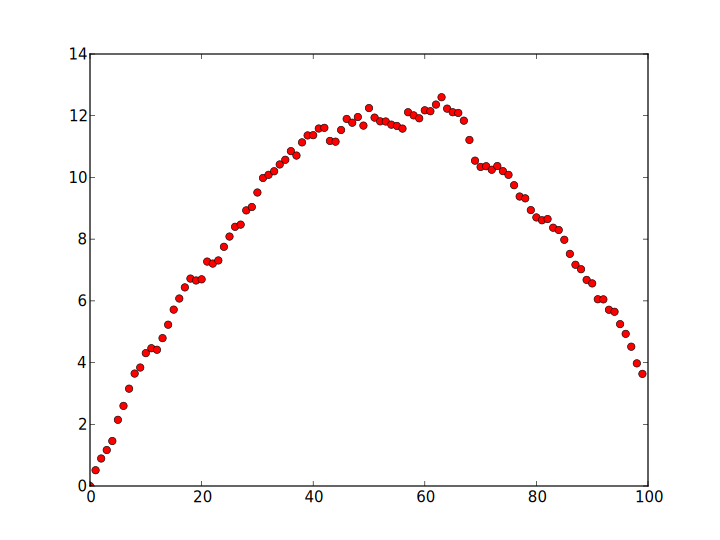
\includegraphics[width=0.5\textwidth,height=\textheight]{AdvFilteringFigures/scalarkalmandata1.*}
\caption{Plot of \(x_0\).}
\end{figure}

\begin{figure}
\centering
\includegraphics[width=0.5\textwidth,height=\textheight]{AdvFilteringFigures/scalarkalmandata2.*}
\caption{Noisy observation of \(x_0\).}
\end{figure}

Using the fake observations, we can test the filter.

\begin{Shaded}
\begin{Highlighting}[]
\NormalTok{x\_filtered }\OperatorTok{=}\NormalTok{ zeros(N)}
\NormalTok{covariance\_filtered }\OperatorTok{=}\NormalTok{ zeros(N)}

\KeywordTok{for}\NormalTok{ k }\OperatorTok{=} \FloatTok{2}\OperatorTok{:}\NormalTok{N}
\NormalTok{   x\_process\_update }\OperatorTok{=}\NormalTok{ x\_filtered[k}\OperatorTok{{-}}\FloatTok{1}\NormalTok{] }\OperatorTok{+} \FloatTok{0.5}\OperatorTok{*}\NormalTok{(N}\OperatorTok{{-}}\FloatTok{1.75}\OperatorTok{*}\NormalTok{u[k])}\OperatorTok{/}\NormalTok{N}
\NormalTok{   variance\_update }\OperatorTok{=}\NormalTok{ covariance\_filtered[k}\OperatorTok{{-}}\FloatTok{1}\NormalTok{] }\OperatorTok{+}\NormalTok{ sigma1}\OperatorTok{*}\NormalTok{sigma1}
\NormalTok{   kal\_gain }\OperatorTok{=}\NormalTok{ variance\_update}\OperatorTok{/}\NormalTok{(variance\_update }\OperatorTok{+}\NormalTok{ sigma2}\OperatorTok{*}\NormalTok{sigma2)}
\NormalTok{   x\_filtered[k] }\OperatorTok{=}\NormalTok{ x\_process\_update }\OperatorTok{+}\NormalTok{ kal\_gain}\OperatorTok{*}\NormalTok{(z\_sim[k}\OperatorTok{{-}}\FloatTok{1}\NormalTok{] }\OperatorTok{{-}}\NormalTok{ x\_process\_update)}
\NormalTok{   covariance\_filtered[k] }\OperatorTok{=}\NormalTok{ (}\FloatTok{1}\OperatorTok{{-}}\NormalTok{kal\_gain)}\OperatorTok{*}\NormalTok{variance\_update}
\KeywordTok{end}

\NormalTok{p3 }\OperatorTok{=}\NormalTok{ plot(u}\OperatorTok{,}\NormalTok{x\_filtered)}
\NormalTok{display(p3)}
\end{Highlighting}
\end{Shaded}

\begin{figure}
\centering
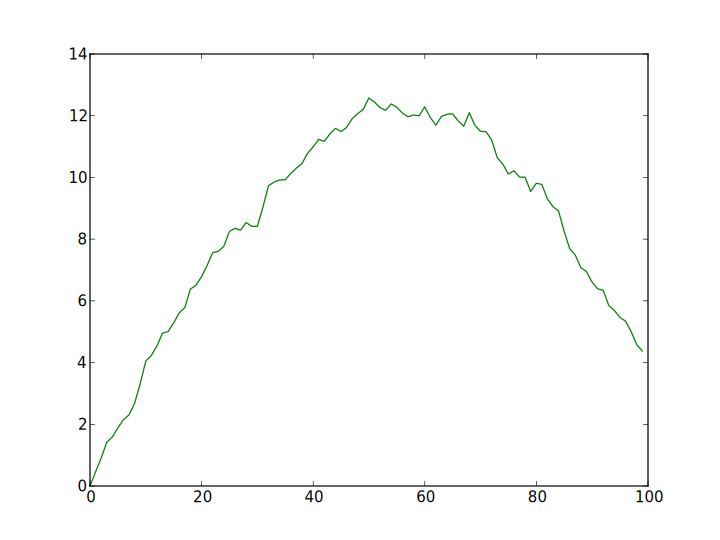
\includegraphics[width=0.5\textwidth,height=\textheight]{AdvFilteringFigures/scalarkalmandata3.*}
\caption{Kalman estimate of \(x_0\).}
\end{figure}

\begin{figure}
\centering
\includegraphics[width=0.5\textwidth,height=\textheight]{AdvFilteringFigures/scalarkalmandata4.*}
\caption{Comparison of state estimate to real state.}
\end{figure}

\textbf{Footnotes}
